% Chapter Template

\chapter{Results - Rubik's Cube} % Main chapter title

\label{sec:ResRubiks} % Change X to a consecutive number; for referencing this chapter elsewhere, use \ref{ChapterX}

%----------------------------------------------------------------------------------------
%	SECTION 1
%----------------------------------------------------------------------------------------

I now discuss my experiments on the Rubik's cube. I have run reasonably comprehensive trial on the 2x2x2, throwing 6 of my solvers at the problem. As mentioned in \ref{sec:Puzzles}, the 2x2x2 \textbf{RC}, in spite of its deceivingly simple physical appearance, is actually not that much easier to solve (by hand) than the 3x3x3. For instance, it takes me usually just under one minute, versus two minutes for the 3x3x3. I am obviously no \textit{speedcuber}, but my time-to-solve and perceived difficulty ratios are in line with that of experienced players who might take 2-3 seconds for the 2x2x2 and 10 seconds for the 3x3x3. Computing wise, the 2x2x2 was of decent size for my purpose, with its 88 million configurations. Table \ref{tab:gridRC} summarizes which solvers I have attempted to run on the 2 dimensions:

\begin{table}[H]
\begin{center}
\begin{tabular}{l*{5}{c}r}
\hline
\textbf{solver}      & & \textbf{Rubik's} & \textbf{2x2x2} & \textbf{3x3x3} \\
\hline
BFS   &   &        &  x  &  x  \\
\hline
Kociemba   &   &      &  x  &  x  \\
\hline
A$^{*}$[Kociemba]  &   &  &  x  &  x  \\
\hline
A$^{*}$[DL[A$^{*}$[Kociemba]]]  &   &  &  x  &  x  \\
\hline
A$^{*}$[DRL]  &   &  &  x  &  \\
\hline
A$^{*}$[DQL]  &   &  &  x  &  \\
\hline
%MCTS[DQL][c=0]  &   &  & x &  \\
%\hline
%MCTS[DQL][c=69]  &   & & x &  \\
%\hline
\end{tabular}
\caption{\label{tab:gridRC} Solvers used vs \textbf{RC} dimension}
\end{center}
\end{table}








\Section{2x2x2}
All the following experiments on the 2x2x2 \textbf{RC} have been run using my Solver's \textit{performance\_test} (see \ref{sec:codesolvers}): for each level of difficulty, the test presents the solvers with the same 100 random configurations (for fairness and to increase the significance of the results). The levels of difficulty (number of scrambles from goal) used here go from 2 to 20 in step of 2. The tests were also run with perfect shuffling (difficulty = $\infty$ on the graphs), corresponding to taking scrambling to $\infty$ as explained in \ref{Theory:222RCSSS}).

\Subsection{BFS}
For \textbf{BFS} I used a step of 1 on the difficulty and stopped at 5 as it was clear it would not go much further. Its run time and expanded nodes are increasing linearly with difficulty, and it was already taking an average close to a minute for 5 shuffles from goal.

\Subsection{Kociemba, A$^{*}$[Kociemba], A$^{*}$[DL[A$^{*}$[Kociemba]]]}
I obviously expected Kociemba (see \cite{HKociemba} and \cite{Kociemba}) to be by far the fastest solver since it is handcrafted with much specific knowledge about the \textbf{RC} group theory and multi-stage solving (see section \ref{Theory:RCMSS}). Contrary to its claims, I found the 2x2x2 library to not be optimal, running A$^{*}$ with Kociemba's cost as a heuristic indeed resulted in shorter solutions. I did however set Kociemba as my benchmark in the \textit{performance\_test} since I had no admissible heuristic to guarantee optimality otherwise. The optimality scores (top-right graph of figure \ref{fig:222RCPerformance}) therefore do reach more than 100\%, as all other solvers found shorter solutions than Kociemba. I used the solutions of A$^{*}$[Kociemba] on perfectly randomly generated configurations to train the \textbf{DL} heuristic. Since Kociemba is itself using a two-stage IDA$^{*}$ solver, I end-up here with 3 levels of nested A$^{*}$ algorithms: A$^{*}$[DL[A$^{*}$[IDA$^{*}$[2-stage-subgroups]]]]!






\Subsection{Deep Reinforcement Learner \& Deep Q Learner}
\label{sec:S33DRL}
To get my \textbf{DRL} and \textbf{DQL} heuristics, I have run the DeepReinforcementLearner and DeepQLearner with the following main parameters:
\begin{itemize}
\item Update the target network every 1,000 epochs (\textit{update\_target\_network\_frequency}) or when $\frac{MSE}{max target}$ falls below 0.1\% (\textit{update\_target\_network\_threshold=1e-3})
\item Stop at \textit{nb\_epochs}=11,000 or if the max target has not increased more than 1\% (\textit{max\_target\_uptick}) in the last 5,500 epochs (\textit{max\_target\_not\_increasing\_epochs\_pct}=0.5)
\item At each target net update (\textit{training\_data\_every\_epoch}=False), generate \textit{nb\_sequences}=10,000 sequences of puzzles comprised of a 15-scramble puzzle along with its path to goal (\textit{nb\_shuffles}=15).
\item Fully connected network (\textit{network\_type=fully\_connected\_net}) with three hidden layers (\textit{layers\_description}=(600,300,100)), an RMSProp optimiser (\textit{optimiser=rms\_prop}), \textit{scheduler=exponential\_scheduler} with \textit{gamma\_scheduler}=0.9999 and \textit{learning\_rate}=0.1\%. The networks architectures are shown in figure \ref{fig:222RCnets}.
\end{itemize}



\begin{figure}[H]
  \noindent
  \makebox[\textwidth]{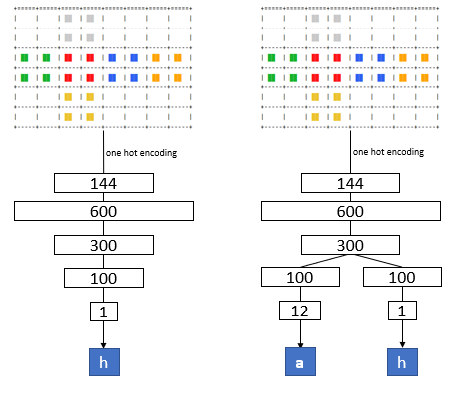
\includegraphics[scale=0.6]{./Figures/222RCnets}}
  \caption[222RCnets]{2x2x2 \textbf{RC} architecture for \textbf{DRL} (left) \& \textbf{DQL} (right) heuristics training}
  \label{fig:222RCnets}
\end{figure}


\noindent Graphs \ref{fig:222RCDRL} and \ref{fig:222RCDQL} show both learners' following metrics tracked over the epochs:
\begin{itemize}
\item learning rate: decreasing due to the scheduler and reset at each network update.
\item max target: an interesting dynamic during learning is that since targets are constructed using value-iteration update, starting from an all 0 network, the max target increases by at most about 1 at every network update, until we reach God's number. The first network only learns to differentiate goal from non-goal, the second one learns how to differentiate goals, cost 1 and cost 2+ \dots. This is why I introduced \textit{update\_target\_network\_threshold} discussed above, to makes sure we do not spend time initially training the left-hand-side network when it is easy. \textit{max\_target\_uptick} and \textit{max\_target\_not\_increasing\_epochs\_pct} make sure that we stop training when the max target does not grow anymore.
\item loss: MSE for \textbf{DRL}, MSE + CrossEntropyLoss for \textbf{DQL}
\item loss divided by max target: the exit criterion \textit{update\_target\_network\_threshold} is based on that quantity, since a loss of e.g. 1\% means little if the we do not compare it to the possible range of the cost-to-go.
\item The percentage of all the possible puzzles of that dimension \textit{seen} by the learner. This is an interesting quantity, as it tells us how well the solvers are able to generalise. From both graphs (\ref{fig:222RCDRL} \& \ref{fig:222RCDQL}) we can see that the learners saw less than 1\% of all puzzles. It is good to keep in mind however that \textit{seen} does not mean really much here since the learning is \textit{unsupervised}. This is quite in contrast to the DeepLearner, whose training data consist of puzzles with their cost-to-go computed by a \textit{teacher} (optimal or other efficient solver).
\end{itemize}


\begin{figure}[H]
  \noindent
  \makebox[\textwidth]{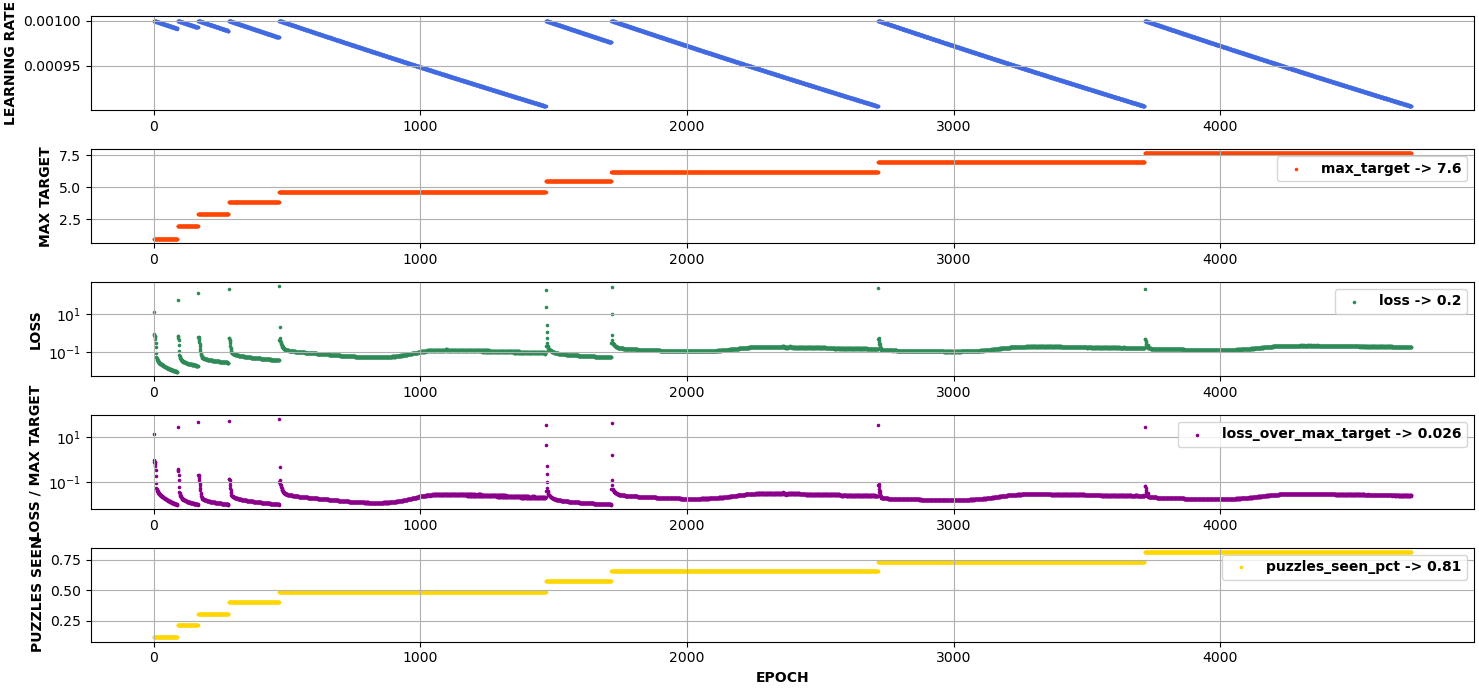
\includegraphics[scale=0.4]{./Figures//222RCDRL}}
  \caption[222RCDRL]{\textbf{DRL} of the 2x2x2 \textbf{RC}}
  \label{fig:222RCDRL}
\end{figure}

\begin{figure}[H]
  \noindent
  \makebox[\textwidth]{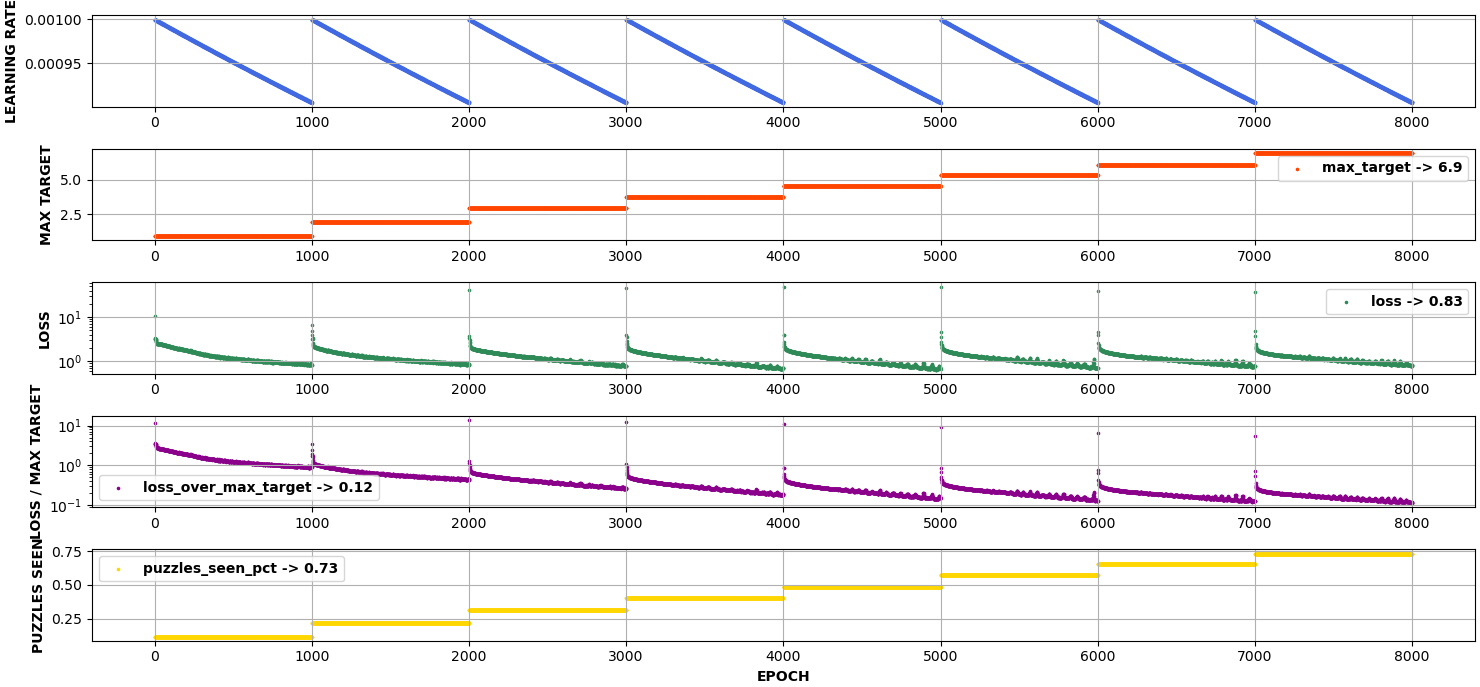
\includegraphics[scale=0.4]{./Figures//222RCDQL}}
  \caption[222RCDQL]{\textbf{DQL} of the 2x2x2 \textbf{RC}}
  \label{fig:222RCDQL}
\end{figure}




\Subsection{Solvers' comparison}

I summarize as usual the 2x2x2 \textbf{RC} performance tests with my usual metrics in figure \ref{fig:222RCPerformance}. Overall, the \textbf{DL} and \textbf{DRL} managed to solve all cubes (though \textbf{DL} took over an hour and \textbf{DRL} 6 hours for their slowest cube. Both methods outperformed Kociemba in terms of optimality-score and got on par with A$^{*}[Kociemba]$. Their max cost over all cubes encountered was 12 for up to 20 shuffles, and 13 for $\infty$ shuffling. Considering God's number for the 2x2x2 \textbf{RC} of 11, this is rather impressive!
\\
\\
Quite remarkably we can see (second graph of \ref{fig:222RCDRL}) that the \textbf{DRL} heuristic only ever assigned a cost-to-go of 7.6 at most. Despite that, it was still able to solve cubes requiring up to 13 moves (likely to have been among the hardest 2x2x2 cubes). How is that possible? Notice that the loss of 0.2 towards which the network converged at the end of its training is misleading, since this is in-sample loss versus the target network. My theory is that while the value the \textbf{DRL} assigned to hard-to-solve cubes can be off (by at least 4 or 5), it is likely that the network gets the relative value of neighbouring cubes right (not that surprising given the value-iteration), and this is sufficient to guide A$^{*}$ extremely well. If both the absolute value of the cost-to-go and the relative (among neighbouring cubes) was totally off, we would indeed not expect the heuristic to make A$^{*}$ any better than, say, \textbf{BFS} and we would therefore not expect it to be able to solve \textit{costly} cubes requiring 10+ moves.
\\
\\
Finally, we can see that \textbf{DQL}, despite showing visually cleaner and more monotonic loss convergence than \textbf{DRL} (see \ref{fig:222RCDQL} versus \ref{fig:222RCDRL}), struggled a lot more to solve difficult cubes (above 10 shuffles). This shows that my earlier findings on the 3x3 \textbf{SP} are likely not universal, and very much depend on the parameters set during training, as well as on the problem at hand.

\begin{figure}[H]
  \noindent
  \makebox[\textwidth]{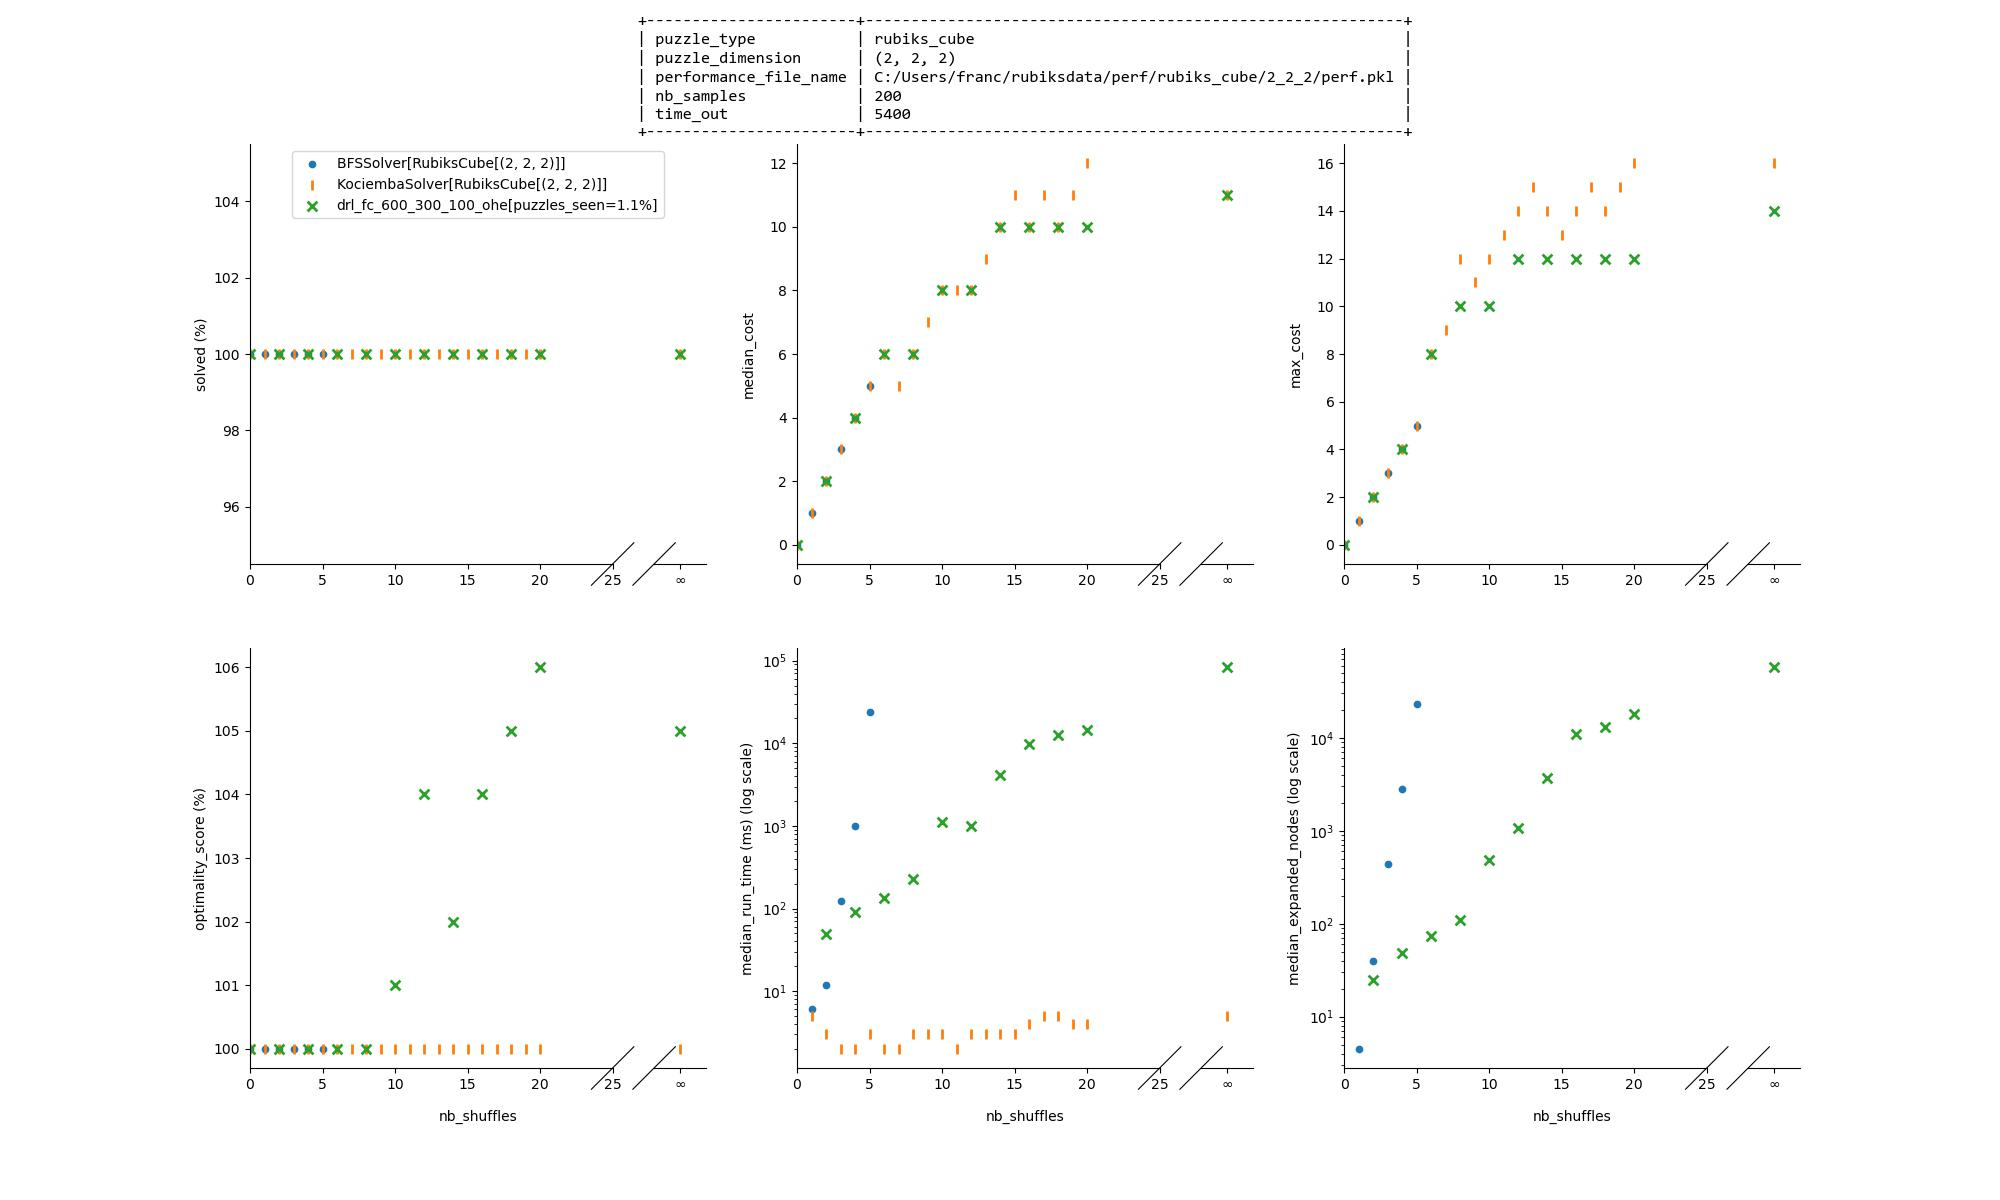
\includegraphics[scale=0.52]{./Figures/222RCPerformance}}
  \caption[222RCPerformance]{Solvers' performance comparison 2x2x2 \textbf{RC}}
  \label{fig:222RCPerformance}
\end{figure}



%-----------------------------------
%	SUBSECTION 1
%-----------------------------------
\Section{3x3x3}
\label{sec:ResRubiks333}

I did not get to run very many experiments on the 3x3x3 \textbf{RC}. The results of the performance test (50 random configurations for levels of difficulty from 2 to 40 by increment of 2 as well as $\infty$ shuffling) can be found on figure \ref{fig:333RCPerformance}.
\begin{itemize}
\item Here again, Kociemba does not show optimality, since we can see that my A$^{*}[Kociemba]$, that is A$^{*}$ using Kociemba as a heuristic, performs much better than Kociemba (solutions about 20\% shorter at $\infty$ shuffling). This is not surprising though since Kociemba 3x3x3 does not claim to be optimal and is meant to find solution in the 40 moves at most (which is what I have observed indeed). A$^{*}[Kociemba]$ never took more than 30 moves on any of the cubes presented to it, which is not bad given the known God number of 26 in the quarter-turn-metric (as discussed earlier in \ref{Theory:333RCSSS})
\item A$^{*}$[\textbf{DL}] managed to solve all puzzles scrambled less than 10 times, and found shorter worst-case solutions than even A$^{*}[Kociemba]$ on which it was trained. Within the 2 hours time-out, it failed to solve one of the 50 cubes for difficulty 10, and two of the 50 cubes of difficulty 12, so i did not try further than that.
\item A$^{*}$[\textbf{DRL}] only managed to solve all puzzles of difficulty less than 6 but at least did find only optimal solutions (compared with \textbf{BFS}).
\end{itemize}


\begin{figure}[H]
  \noindent
  \makebox[\textwidth]{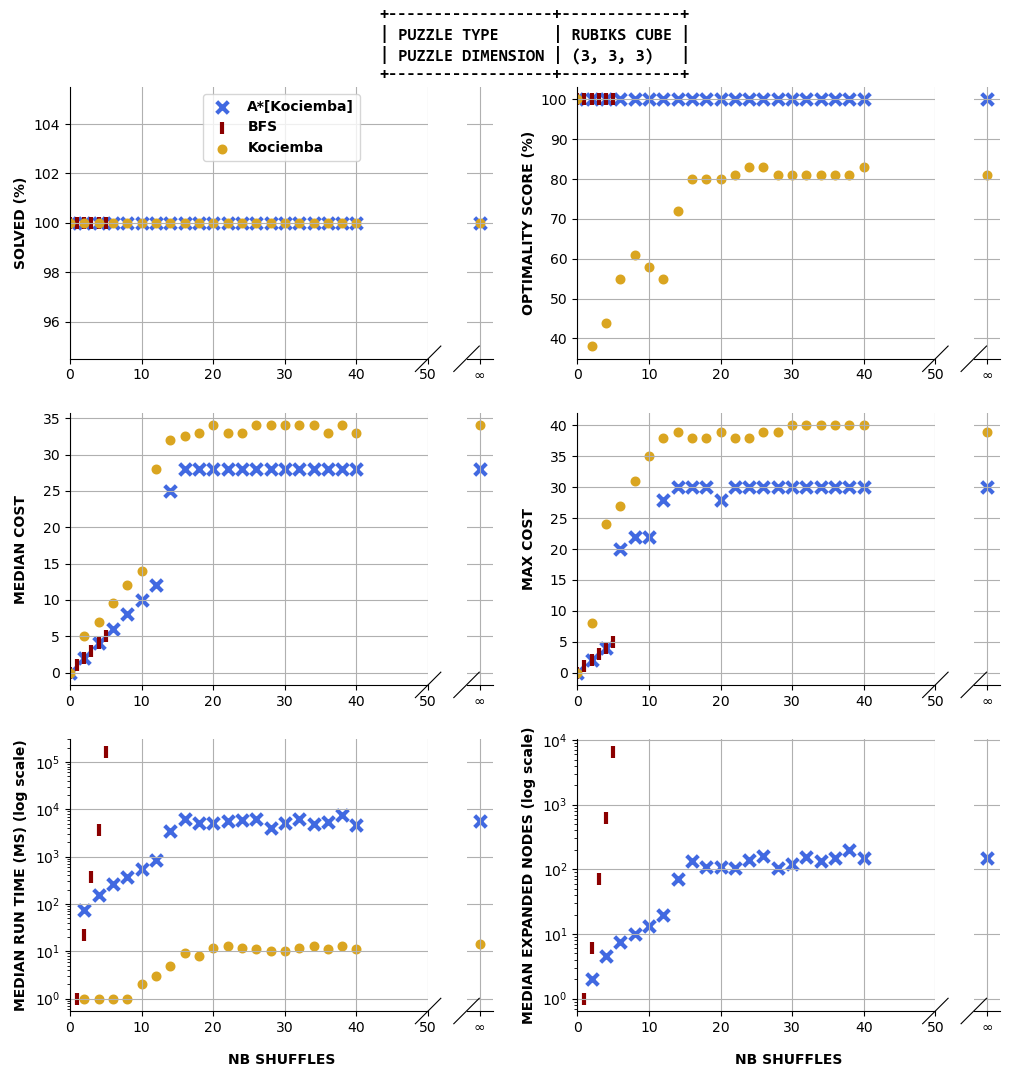
\includegraphics[scale=0.52]{./Figures/333RCPerformance}}
  \caption[333RCPerformance]{Solvers' performance comparison 3x3x3 \textbf{RC}}
  \label{fig:333RCPerformance}
\end{figure}
